%% ----------------------------------------------------------------------------------
%% GUIDELINES
%% ----------------------------------------------------------------------------------
%% - Provide details about techniques/methods that you use. Do not just write “We have
%% implemented the marching cubes algorithm”. Describe the method too, in your own
%% words. Even if it is well described in a book, you should still explain the method
%% yourself; this is part of the exercise. Also, the reader may not know the method, nor
%% can the reader be bothered to find the document that you are referring to.
%% - Discuss interesting implementation aspects, but do not include code fragments in the
%% text. Pseudo code is allowed, but mathematical formulas are preferred.
%% - Describe parameters of methods and explain which settings you used and why.
%% - Provide evidence that the method you have implemented actually works as intended.
%% - Explain how you designed a color map, a transfer function, or even your whole visualization
%% approach.

\section{MIP}\label{sec:mip}
We will start this section with explaining how the MIP raycaster was developed from the initially provided application. The initial code simply used to take a slice (plane) through the data. This plane would go through the exact center of the bounding box, and would be tilted in order to be perpendicular to the view vector \texttt{viewVec} at all times. In order to let the raycaster perform MIP, we need not only to consider the data on the slice plane, but for each pixel we need to consider all of the data on the ray from that pixel parallel to \texttt{viewVec}. We then take the maximum of these values, and project that value onto the corresponding pixel. From an implementation point of view this means that we need to introduce an additional for-loop that walks along the described ray for every pixel. 


- add the depth part rather than just plane
- diagonal is diagonal of the bounding box

\subsection{Tri-linear Interpolation}\label{subsec:tri_linear}
- added function getTriVoxel
- %http://en.wikipedia.org/wiki/Trilinear_interpolation

\begin{figure}[h!]
    \centering
    \captionsetup{justification=centering,margin=0.5cm}
    \begin{subfigure}[t]{0.48\textwidth}
        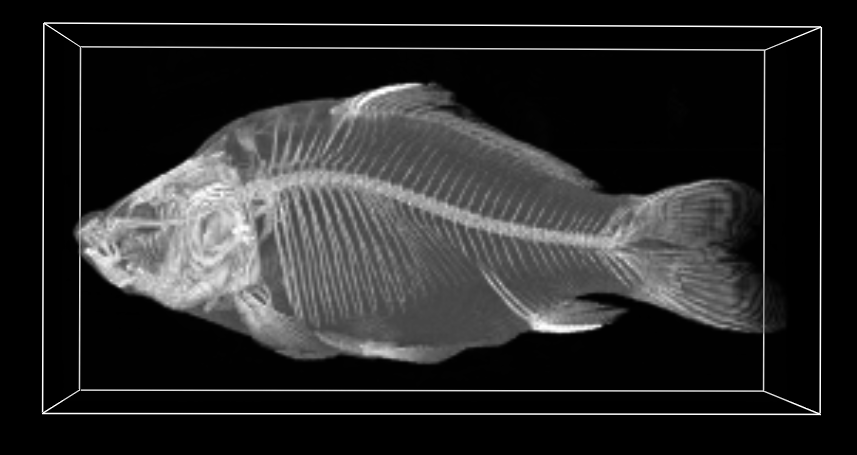
\includegraphics[width=\textwidth]{img/fish_NN.png}
        \caption{ }
    \end{subfigure}
    \begin{subfigure}[t]{0.48\textwidth}
        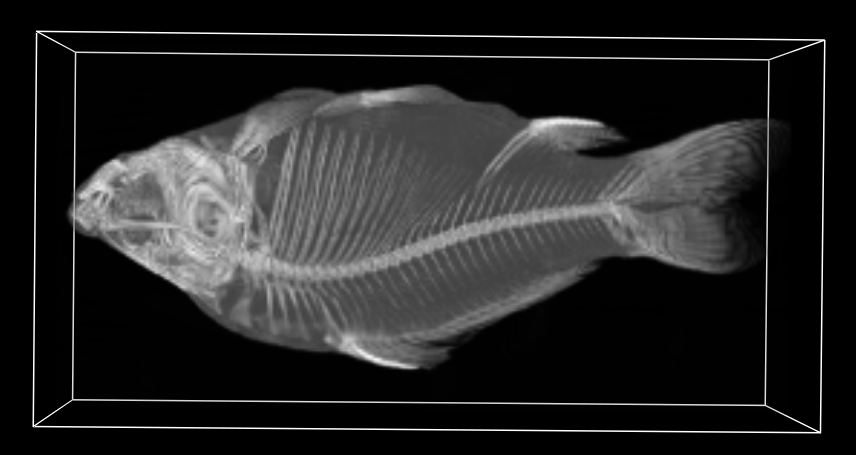
\includegraphics[width=\textwidth]{img/fish_TriLin.png}
        \caption{ }
    \end{subfigure}
    \caption{difference between NN interpolation and Tri-Linear interpolation}
    \label{fig:trilinear}
\end{figure}

\subsection{Performance Enhancing}\label{subsec:perf_enh}

- took location calculation for i and j out of the k-for-loop
- let loop break when a value of 255 is already found (can't get any higher) (does not work for composite though)
%- todo: compute the length of the ray before entering the k-loop (depth-loop)
- wanted to decrease length of 'depth' for-loop but already checked within getVoxel method.
- bring back resolution when rotating
- 

